\chapter{Conclusiones}

\section{Resultados}

\section{Problemas Encontrados}

El principal problema, a la hora de desarrollar el proyecto ha sido el uso de datos de geolocalización en la aplicación. Debido a temas de privacidad por parte de los usuarios, un porcentaje superior al 90\% no tenía activada la geolocalización en su aplicación de Twitter. De modo que para representar la información en el mapa de la aplicación, se obtenía la ciudad del usuario al que pertenecía el Tweet.

\vspace{5 mm}

De esta forma los tweets que eran de la misma ciudad se solapaban en un mismo punto (las coordenadas centrales de la ciudad). De modo que para que se visualizarán los datos en el mapa sin solapamiento se decidió por generar dos números aleatorios, uno para la latitud y otro para la longitud, que estuviera dentro del rango de los limites de la ciudad delimitados por Google Maps.

\vspace{5 mm}

Este método consiguió solucionar la forma de visualizar los datos en el mapa. Aunque los datos no se podrían considerar 100\% fiables, ya que se falsean los datos. No se puede saber con exactitud la proveniencia de los tweets. Un ejemplo de este caso sería el de un usuario de Alicante, que podría estar twitteando desde Madrid.


\section{Mejoras y ampliaciones}

La principal mejora a implementar se encuentra en el rediseño de la arquitectura de la aplicación. Para conseguir una web con más dinamismo e interacción con el usuario se utilizará el framework de javascript Angularjs.Además Este framework, permite generar un patrón de MVC que permite programar el front-end de la aplicación más modular y tener el código mejor estructurado.

\vspace{5 mm}

En cuanto a la parte de back-end, se deberá refactorizar el código de forma que sea escalable para una implementación real, donde la cantidad de información y el número usuarios es bastante superior al prototipo funcional. 

\vspace{5 mm}

También se tendrán que utilizar herramientas de Big Data, ya que actualmente los datos se gestionan desde un cliente de bases de datos \cite{big-data-tools}. 
Existen muchas herramientas de Big Data, y están especializadas en un área, se necesitarán algunas tales como:


\begin{itemize}
  \item \textbf{Hadoop}, una herramienta de almacenado. Un framework open-source que permite trabajar con miles de petabytes de datos.
  \item \textbf{Oracle data mining},herramienta de mineria de datos muy potente. Permite hacer predicciones acerca de los datos y crear modelos para descubrir el comportamiento del cliente.
  \item \textbf{Chartio}, herramienta de visualización. Te permite crear potentes gráficas y paneles de visualización de datos en unos pocos clicks.
\end{itemize}

\section{Modelo de negocio}

\begin{figure}
\begin{center}
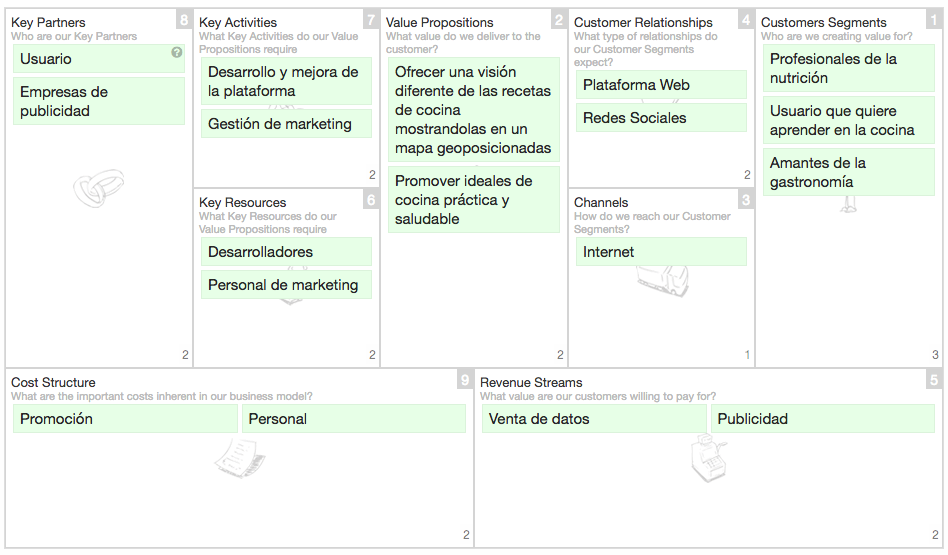
\includegraphics[width=1.0\textwidth]{imagenes/business-canvas.png}
\caption{Listado de elementos}
\label{business-canvas}
\end{center}
\end{figure}

Despues de desarrollar un producto mínimo viable de la aplicación de Njoycooking, se plantea la siguiente cuestión: ¿Es posible generar un modelo de negocio para la aplicación?

Mediante un business model canvas(figura \ref{business-canvas}) se describe de una forma simple en que consiste la idea de negocio.

\vspace{5 mm}

Al generar un modelo de negocio, el primer concepto que se tiene que valorar es: ¿Qué propuesta de valor ofrece la aplicación? es decir que elemento diferenciador puede ofrecer la aplicación frente otros existentes en el mercado. NjoyCooking es una aplicación gastronómica pero además de ofrecer un blog de cocina proporciona un visión diferente de los recetas de cocina, mostrando lo que cocina la gente según su zona geográfica mostrando las recetas geoposicionadas en un mapa y en tiempo real. Otra propuesta, es la de promover los hábitos de cocina práctica y saludable. 


\vspace{5 mm}

Otro concepto que se tiene que valorar es como relacionarse con el cliente. El principal punto de contacto con los clientes será la aplicación web, donde los usuarios podrán interactuar y conocer la propuesta de valor que ofrece. Otra forma de contactar será mediante las redes sociales, ya que son un medio de difusión muy importante para a dar a conocer la aplicación.

\vspace{5 mm}

¿De dónde se obtendrán los ingresos? Las principales fuentes de ingresos serán dos:

\begin{description}

\item [Publicidad:] se proporcionará a las empresas la posibilidad de anunciarse en el sitio web mediante banners.

\item \textbf{Venta de datos}: los datos recogidos en la aplicación se ofrecerán a cambio de un pago económico a las empresas interesadas. Estos datos pueden servir a las empresas, que pueden realizar un estudio de mercado con ellos en función de las gustos y preferencias que tienen los usuarios de NjoyCooking.

\end{description} 

\vspace{5 mm}

¿Cuales son las fuentes clave? ¿Es decir que personal se necesita para llevar a cabo la propuesta de valor? Para cumplir la propuesta de valor se necesitará la contratación de programadores de software para desarrollar y mejorar la aplicación y especilistas en marketing para dar a conocer la aplicación y ofrecer un mejor uso y experiencia de ella.

\vspace{5 mm}

El usuario activo de la aplicación será el principal partner de la aplicación, ya que podrá promover la plataforma a sus conocidos y así abarcar un mayor número de usuarios. Las empresas de marketing y publicidad también se tienen en cuenta ya que pueden ayudar a llevar a cabo la propuesta de valor patrocinando el producto.


\vspace{5 mm}

Por último se debe tener en cuenta: ¿A qué público va enfocada la propuesta de valor? NjoyCooking tiene como objetivo un público concreto como son los amantes de la gastronomía y cocina en general. Aunque el objetivo es específico, engloba un abánico de usuarios amplio donde existe una variedad por edad,sexo,profesión o aptitudes culinarias.



